\begin{landscape}
\subsubsection{Vergleich Features}
\renewcommand{\arraystretch}{1.5}
% --- Vergleich Features, Teil 1 ---
\begin{longtable}{p{2.8cm}p{3.5cm}p{3.5cm}p{3.5cm}p{3.5cm}p{3.5cm}}

	% Header
	& \rotatebox{90}{LG G Watch} 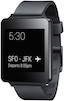
\includegraphics{Bilder/SmartWatch/lg_g_watch}
	& \rotatebox{90}{LG G Watch R} 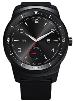
\includegraphics{Bilder/SmartWatch/lg_g_watch_r}
	& \rotatebox{90}{LG Watch Urbane LTE} 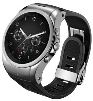
\includegraphics{Bilder/SmartWatch/lg_watch_urbane_lte}
	& \rotatebox{90}{Motorola Moto 360} 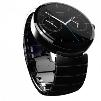
\includegraphics{Bilder/SmartWatch/moto_360}
	& \rotatebox{90}{Apple Watch} 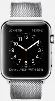
\includegraphics{Bilder/SmartWatch/apple_watch}\\
	\hline
	\endfirsthead
	
	\multicolumn{3}{l}{Fortsetzung} \\
	& {LG G Watch}
	& {LG G Watch R}
	& {LG Watch Urbane LTE}
	& {Motorola Moto 360}
	& {Apple Watch} \\
	\hline
	\endhead

	% Content
	Display
		& 1.65 Zoll \newline
			280x280px (204ppi) \newline
			IPS
		& 1.3 Zoll \newline
			320x320px (245ppi) \newline
			P-OLED
		& 1.3 Zoll \newline
			320x320px (245ppi) \newline
			P-OLED
		& 1.56 Zoll \newline
			320x290 (205ppi) \newline
			IPS
		& 1.32 Zoll \newline
			272x340 \\
	Prozessor
		& 1,2-GHz \newline Snapdragon 400
		& 1,2-GHz \newline Snapdragon 400
		& 1,2-GHz \newline Snapdragon 400
		& 1-GHz \newline Texas Instrument\newline OMAP 3
		& Apple S1 (SIP)\newline System in a package \\
	RAM
		& 512 MB
		& 512 MB
		& 1 GB
		& 512 MB
		& 512 MB ?\\
	interner Speicher
		& 4 GB
		& 4 GB
		& 4 GB
		& 4 GB
		& 4 GB / 8 GB ?\\
	Akku
		& 400 mAh
		& 410 mAh
		& 700 mAh
		& 320 mAh
		& NA\\
	Betriebssystem
		& Android Wear
		& Android Wear
		& LG Wear Platform \newline (ehem. HP WebOS)
		& Android Wear
		& Watch OS \\
	Kompatibilität
		& Android 4.3+
		& Android 4.3+
		& Autonom
		& Android 4.3+
		& iOS 8+\\
	Netzwerk
		& -
		& -
		& LTE
		& - 
		& -\\
	Verbindung
		& BLE 4.0
		& BLE 4.0
		& BLE 4.0 \newline
			Wifi 802.11 b/g/n \newline
			NFC
		& BLE 4.0 \newline
			WiFi (disabled)
		& BLE 4.0 \newline
			WiFi 802.11 b/g/n \newline
			NFC \\
	Schnittstellen
		& Mikrofon
		& Mikrofon
		& Mikrofon \newline
			Lautsprecher
		& Mikrofon
		& Mikrofon \newline
			Lautsprecher \\
	Sensoren
		& Beschleunigungssensor \newline
			Gyroskop \newline
			Kompass \newline
			Schrittzähler
		& Herzfrequenz \newline
        		Beschleunigungssensor \newline
			Gyroskop \newline
			Kompass \newline
			Schrittzähler
		& Herzfrequenz \newline
        		Beschleunigungssensor \newline
			Gyroskop \newline
			Kompass \newline
			Schrittzähler \newline
			Luftdrucksensor
		& Herzfrequenz \newline
		    Beschleunigungssensor \newline
			Gyroskop \newline
			Kompass \newline
			Schrittzähler
		& Beschleunigung \newline
			GPS \newline
			Gyrometer \newline
			Herzfrequenz \newline
			Kompass \newline
			Multi \& ForceTouch \newline
			Schrittzähler \\
	Sonstiges
		& IP67 \newline
			Always-On Display
		& IP67
		& IP67
		& IP67
		& spritzwassergeschützt \\
	Abmessung
		& 37.9 x 45.6 x 9.95 mm
		& 46.4 x 53.6 x 11.1 mm
		& 46 x 52 x 10.9 mm
		& 46 x 46 x 11.5 mm
		& na\\
	Gewicht
		& 63g
		& 62g
		& 45 - 115g
		& 49 - 124g
		& na\\ 
	Markteinführung
		& Jun 2014
		& Nov 2014
		& na 
		& Sep 2014
		& Apr 2015\\
	Preis\footnote{Preise von digitec.ch (günstigstes Modell), Stand: 17.03.2015}
		& CHF 99.00
		& CHF 199.00
		& na
		& CHF 199.00
		& na \\
	\hline
	\caption{Vergleich Features von Smartwatches, Teil 1} \\
\end{longtable}
\newpage

% --- Vergleich Features, Teil 2 ---
\begin{longtable}{p{2.8cm}p{3.5cm}p{3.5cm}p{3.5cm}p{3.5cm}p{3.5cm}}

	% Header
	& \rotatebox{90}{Huawei Watch} 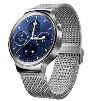
\includegraphics{Bilder/SmartWatch/huawei_watch}
	& \rotatebox{90}{Sony SmartWatch 3} 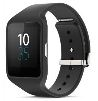
\includegraphics{Bilder/SmartWatch/sony_smartwatch_3}
	& \rotatebox{90}{Samsung Gear S} 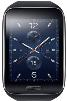
\includegraphics{Bilder/SmartWatch/samsung_gear_s}
	& \rotatebox{90}{Samsung Gear Live} 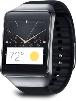
\includegraphics{Bilder/SmartWatch/samsung_gear_live}
	& \rotatebox{90}{Asus ZenWatch} 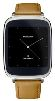
\includegraphics{Bilder/SmartWatch/asus_zen_watch} \\
	\hline
	\endfirsthead
	
	\multicolumn{3}{l}{Fortsetzung} \\
	& {Huawei Watch}
	& {Sony SmartWatch 3}
	& {Samsung Gear S}
	& {Samsung Gear Live}
	& {Asus ZenWatch} \\
	\hline
	\endhead	

	% Content
	Display
		& 1.4 Zoll \newline
			400x400 (286ppi) \newline
			AMOLED
		& 1.6 Zoll \newline
			320x320px
		& 2 Zoll \newline
			480x360px (300ppi) \newline
			Super AMOLED
		& 1.63 Zoll \newline
			320x320px (278ppi) \newline
			Super AMOLED
		& \newline
			320x320px (278ppi) \newline
			AMOLED \\
	Prozessor
		& 1.2 GHz \newline
			Snapdragon 400 \\
	RAM
		& 512 MB
		& 512 MB
		& 512 MB
		&
		&\\
	interner Speicher
		& 4 GB
		& 4 GB
		& 4 GB
		&
		&\\
	Akku
		& 300 mAh
		& 420 mAh 
		& 300 mAh
		& 300 mAh
		& -\\
	Betriebssystem
		& Android Wear
		& Android Wear
		& Tizen 
		&
		& Android Wear \\
	Kompatibilität
		& Android 4.3+
		& Android 4.3+
		& Android 4.3+
		&
		& Android 4.3+ \\
	Netzwerk
		&
		&
		& 
		&
		& \\
	Verbindung
		&
		& BLE 4.0 \newline
			NFC
		&
		& BLE 4.0
		& \\
	Schnittstellen
		&
		& Mikrofon \newline
			Lautsprecher
		&
		& Mikrofon \\
	Sensoren
		& Beschleunigungssensor \newline
			Gyrometer \newline
			Herzfrequenz \newline
			Schrittzähler
		& Beschleunigungssensor \newline
			Gyrometer \newline
			Kompass \newline
			GPS
		& Beschleunigungssensor \newline
			GPS \newline
			Gyrometer \newline
			Helligkeitssensor\newline			
			Herzfrequenz \newline
			(Multi-)Touch
		& Beschleunigungssensor \newline
			Gyrometer \newline
			Herzfrequenz \newline
			(Multi-)Touch \newline
			Schrittzähler \\
	Sonstiges
		&
		& IP68
		& IP67 \newline
			Kopfhörerbuchse
		&
		& IP55\\
	Abmessung
		\\
	Gewicht
		&
		& 45g
		&
		& 59g
		& \\ 
	Markteinführung
		\\
	Preis\footnote{Preise von digitec.ch (günstigstes Modell), Stand: 17.03.2015}
		&		
		& CHF 229.00
		& CHF 329.00
		& -
		& CHF 249.00\\
	\hline
	\caption{Vergleich Features von Smartwatches, Teil 2} \\
	
\end{longtable}
\end{landscape}